% This file is a template using the "beamer" package to create slides for a talk or presentation
% - Talk at a conference/colloquium.
% - Talk length is about 20min.
% - Style is ornate.


% draft包的作用是在编译时不生成目录、图片、超链接等,只处理文字和排版(未显示内容用同等大小的灰色方框替代)
% 这样可以在编辑文档查看效果时加快编译速度
% 但是在确定文档内容后,需要删除draft包(使用下一行documentclass),否则目录不会生成。
% \documentclass[aspectratio=169, UTF8, draft]{beamer}
\documentclass[aspectratio=169, UTF8]{beamer}

\usepackage{ctex} % 中文支持
\usepackage{multicol} % 多栏支持
\usepackage{listings} % 代码高亮
\usetheme{Kokura}

\usepackage[english]{babel} % 在toc中显示英文

% 在封面页需要展示的信息
\title{\textbf{基于Cesium的实景三维专题表达方法研究}}
\subtitle{一份毕业答辩Beamer演示文稿示例} % 可选
\author{Falldio}
\institute{武汉大学资源与环境科学学院}
\date{2021年5月6日}

% Delete this, if you do not want the table of contents to pop up at
% the beginning of each subsection:
% \AtBeginSubsection[]
% {
  % \begin{frame}<beamer>{Outline}
    % \tableofcontents[currentsection,currentsubsection]
  % \end{frame}
% }

\begin{document}
% 默认在title page中加入图片background.png
{
  \usebackgroundtemplate{\includegraphics[width=\paperwidth]{background.png}} % 背景图片
  \begin{frame}[plain, noframenumbering]
    \titlepage
  \end{frame}
}

% 如果不需要背景图片,可以使用下面的命令
% \begin{frame}[plain, noframenumbering]
  % \titlepage
% \end{frame}

% 目录自动生成,显示所有的section和subsection
\begin{frame}[plain, allowframebreaks, noframenumbering]{目录}
  % \begin{multicols}{2} % 多栏显示
  %   \tableofcontents[]%
  % \end{multicols}
  % 如果想要单栏显示目录,可以使用下面的命令
  \tableofcontents
\end{frame}

% 内容主体
\section{研究背景}

\begin{frame}{研究背景与意义}
\end{frame}
\section{理论方法}

\subsection{分栏显示}
\begin{frame}{经典的双栏显示,一边图片一边文字}
    \begin{columns}
        \begin{column}{0.5\textwidth}
            人为分栏可通过columns语法实现\\
            双栏的宽度比例可以通过参数调整\\

        \end{column}
        \begin{column}{0.5\textwidth}
            \begin{figure}[h]
                \centering
                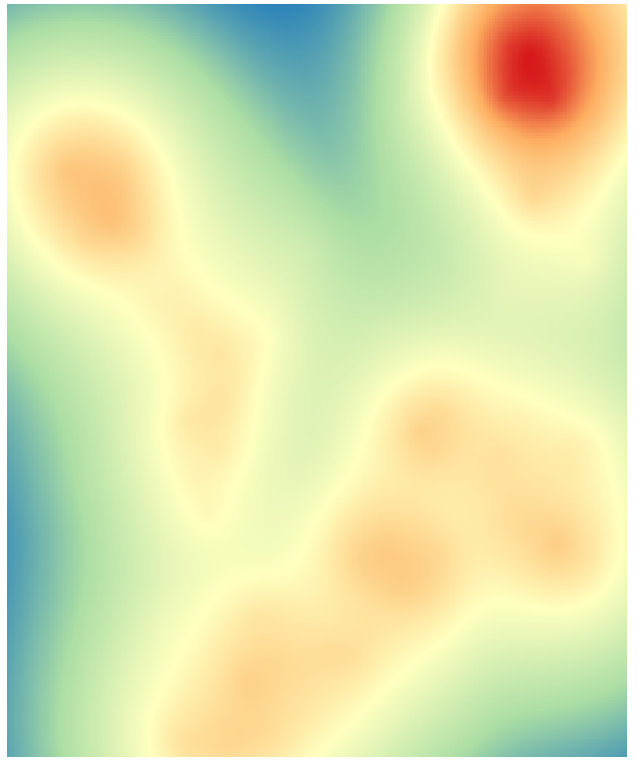
\includegraphics[width=0.5\textwidth]{images/example.png}
                \caption{一张简单的图片示例}
                \label{fig:3dtiles}
            \end{figure}
        \end{column}
    \end{columns}
\end{frame}

\subsection{列表}
\begin{frame}{不带编号的列表}
    使用itemize环境,使用item命令添加列表项
    \begin{itemize}
        \item 1
        \item 2
        \item 3
    \end{itemize}
\end{frame}

\begin{frame}{带有编号的列表}
    使用enumerate环境,使用item命令添加列表项
    \begin{enumerate}
        \item 1
        \item 2
        \item 3
    \end{enumerate}
\end{frame}

\subsection{数学公式}
\begin{frame}{数学公式}
    简单的数学公式使用\$...\$包裹,复杂的公式使用equation环境
    \begin{equation}
        \label{eq:1}
        \sum_{i=1}^n a_i=0
    \end{equation}
\end{frame}
\section{实验过程}

\begin{frame}{研究区域}
\end{frame}
\section{总结展望}

\begin{frame}{总结展望}
\end{frame}

% 致谢页面
{
    \usebackgroundtemplate{\includegraphics[width=\paperwidth]{background.png}} % 背景图片
    \usebeamercolor{structure}
    \begin{frame}[plain]
        \begin{center}
            \textcolor{fg}{\Huge \textbf{敬请各位老师批评指正!}}
            \vskip 1cm
            \textcolor{fg}{\large 焚膏油以继晷,恒兀兀以穷年。}
        \end{center}
    \end{frame}
}

\end{document}


